\documentclass[../NormeDiProgetto.tex]{subfiles}
\begin{document}
	\section{Processi organizzativi}
		\subsection{Scopo}
			Lo scopo dei processi è quello di produrre il \pianodiprogettoRR, al fine di pianificare e
			gestire i ruoli che i membri dovranno assumere nella dinamica della progettazione di
			\progetto.
		\subsection{Aspettative}
			I risultati ottenuti in seguito ad una corretta attuazione di tali processi sono:
			\begin{itemize}
				\item Definire i ruoli dei membri del gruppo;
				\item Pianificare e calendarizzare l'esecuzione dei compiti programmati;
				\item Produrre il \pianodiprogetto.
			\end{itemize}
		\subsection{Gestione organizzativa}
			\subsubsection{Ruoli di progetto}
				L'assegnazione dei ruoli viene pianificata all'interno del \pianodiprogetto. Le ore di
				lavoro devono essere distribuite in modo più possibile omogeneo tra i membri del
				gruppo. Ogni membro deve inoltre ricoprire ciascun ruolo almeno una volta.
				\paragraph{Responsabile di progetto\\}
					Il \responsabilediprogetto\ è il portavoce nonché il responsabile delle scelte
					del gruppo. In particolare si occupa di:
					\begin{itemize}
						\item Approvare l'offerta economica;
						\item Gestire le risorse;
						\item Pianificare e coordinare le attività;
						\item Analizzare e gestire i rischi;	
						\item Approvare i documenti;
						\item Assicurarsi che vengano rispettate le \normediprogetto;
						\item Assicurarsi che vengano rispettate le pianificazioni definite nel
						\pianodiprogetto.
					\end{itemize}
				\paragraph{Amministratore\\}
					L'\amministratore\ è colui che si occupa di gestire l'efficienza dell'ambiente
					di lavoro. In particolare si occupa di:
					\begin{itemize}
						\item Studiare e fornire strumenti che migliorano l'ambiente di lavoro;
						\item Gestire l'archiviazione, il versionamento e la configurazione dei
						documenti e del software;
						\item Eliminare o ridurre per quanto possibile le difficoltà nella gestione
						di processi e di risorse;
						\item Automatizzare il lavoro dove possibile.
					\end{itemize}
				\paragraph{Analista\\}
					L'\analista\ deve identificare e tracciare il dominio del problema.
					In particolare si occupa di:
					\begin{itemize}
						\item Trasformare le richieste del cliente in specifiche per il prodotto;
						\item Elaborare le specifiche nell'\analisideirequisiti\ e nello
						\studiodifattibilita.
					\end{itemize} 
				\paragraph{Progettista\\}
					Il principale ambito di lavoro del \progettista\ è lo \gl{stack tecnologico}.
					In particolare si occupa di:
					\begin{itemize}
						\item Indicare le tecnologie più idonee allo sviluppo del progetto;
						\item Descrivere il funzionamento del sistema e progettarne l'architettura;
						\item Produrre una soluzione ammissibile in termini di risorse impiegate.
					\end{itemize}	
				\paragraph{Programmatore\\}
					Il \programmatore\ è l'addetto alla codifica. In particolare si occupa di:
					\begin{itemize}
						\item Implementare le soluzioni indicate dal \progettista;
						\item Scrivere codice opportunamente commentato, versionato e mantenibile, in
						accordo al documento \normediprogetto;
						\item Stilare la documentazione del codice;
						\item Realizzare e fornire gli strumenti per la verifica e la validazione
						del prodotto.
					\end{itemize}
				\paragraph{Verificatore\\}
					Il \verificatore\ è l'addetto a tutte le attività di verifica.
					In particolare si occupa di:
					\begin{itemize}
						\item Controllare che le regole stabilite dalle \normediprogetto\ siano
						rispettate durante ogni attività di progetto.
					\end{itemize}
				
				
				
				\subsection{Strumento di coordinamento}
				\begin{figure} [h!]
					\centering
					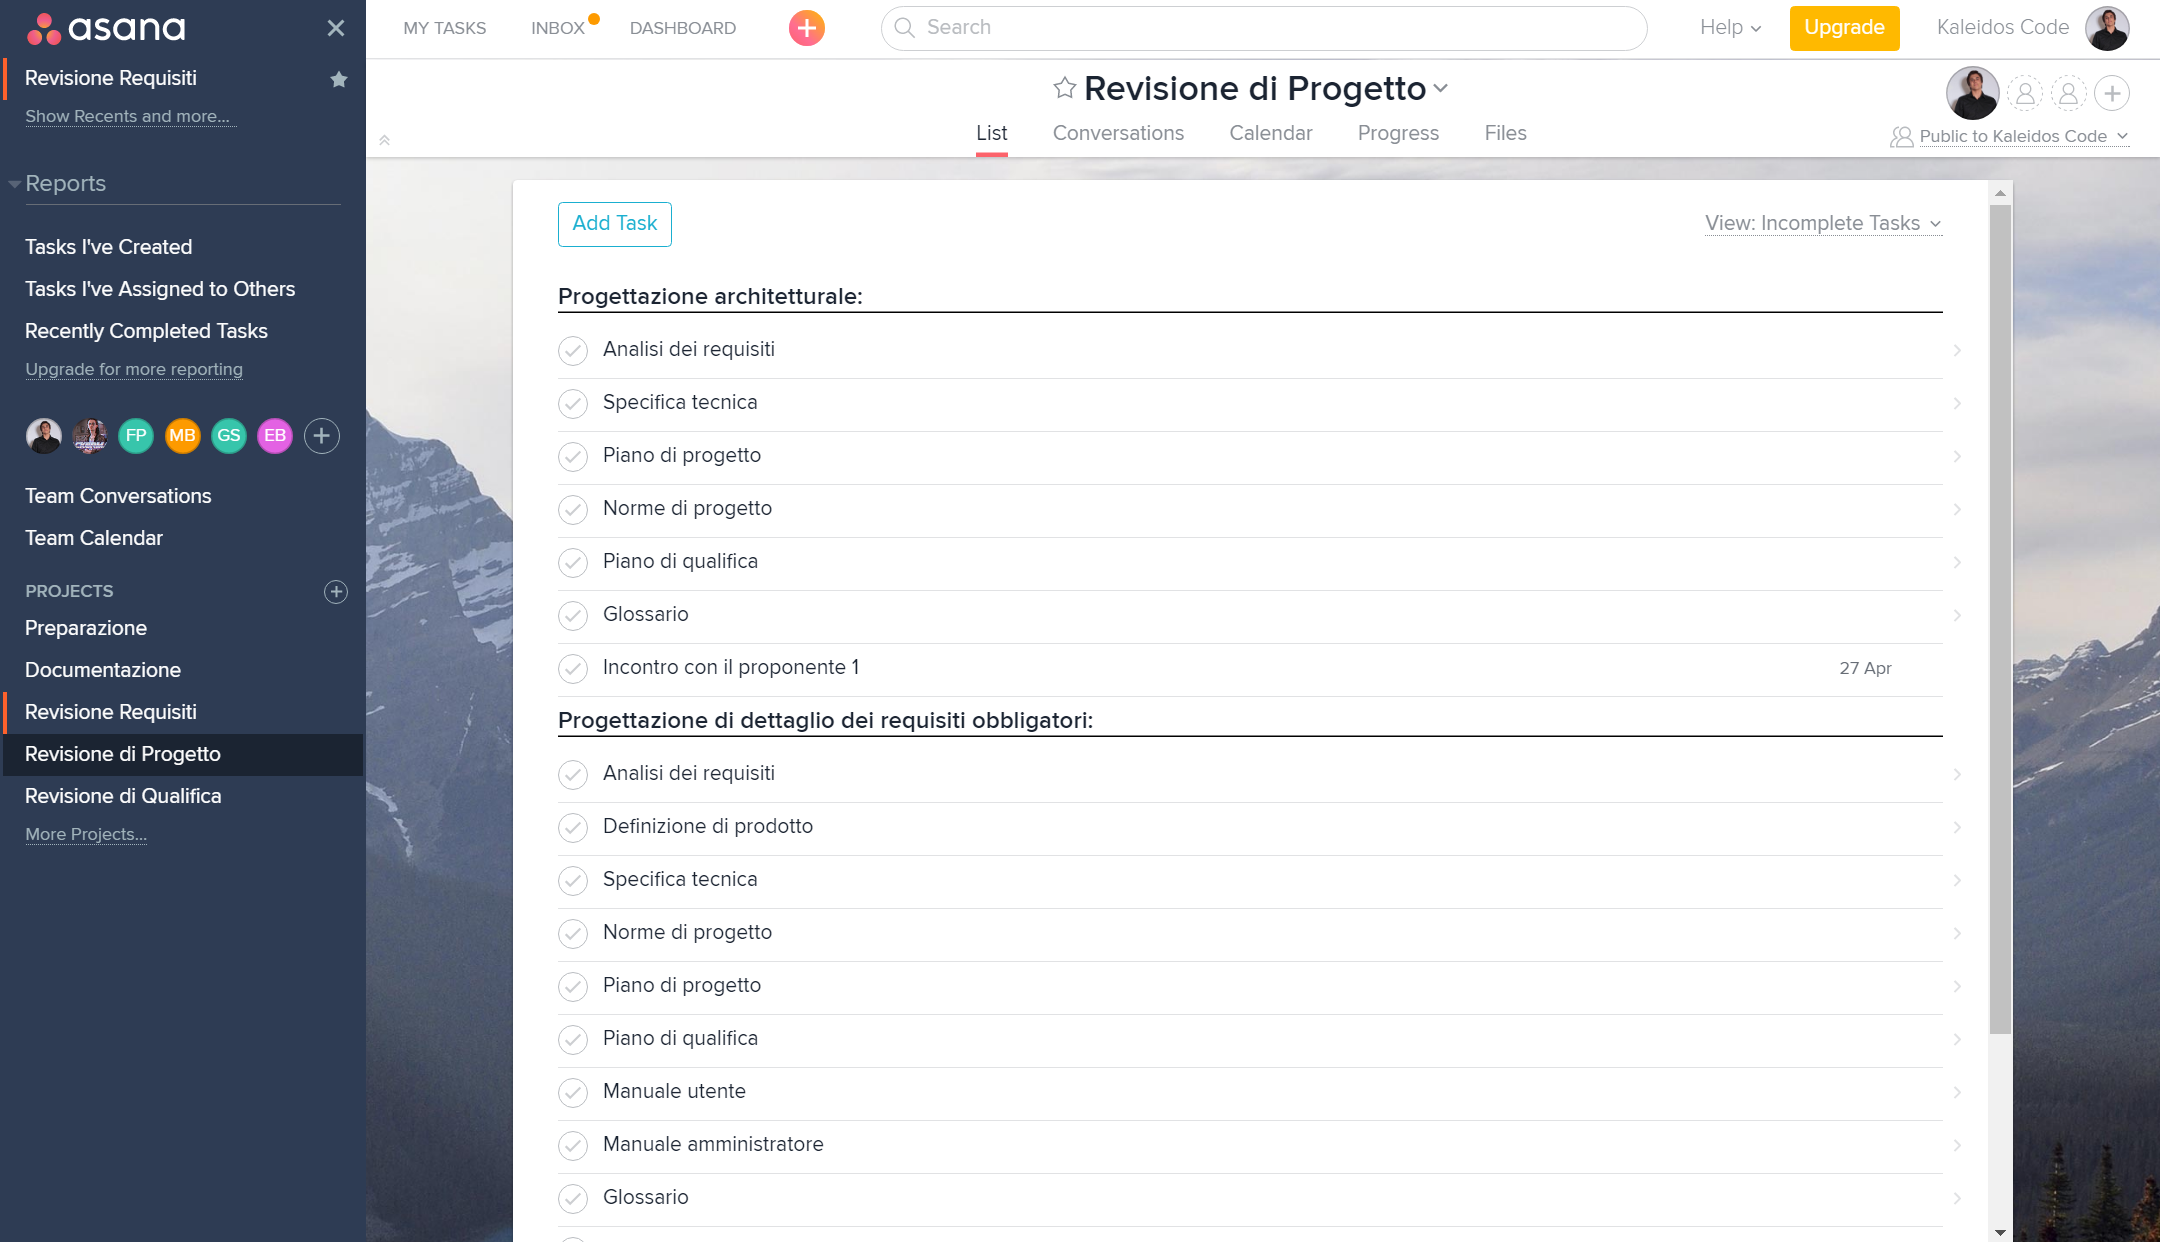
\includegraphics[scale=0.2]{./Immagini/Asana.png}
					\caption{Lista di Task in Asana}\label{}
				\end{figure}
				Come piattaforma di gestione del gruppo è stato scelto \gl{\textbf{Asana}}. Asana fornisce:
				\begin{itemize}
					\item Un sistema di gestione dei task;
					\item Un calendario per organizzare i compiti;
					\item La visualizzazione del repository associato al progetto;
					\item Un sistema di rendicontazione del tempo;
					\item La possibilità di integrare Google Drive, GitHub e web app come Instagantt.
				\end{itemize}
				Sono state valutate diverse alternative ma, dopo un'attenta fase di test, nessuna di queste è
				stata ritenuta all'altezza di Asana per quantità e qualità delle caratteristiche proposte.\\
				Sono stati provati i seguenti software:
				\begin{itemize}
					\item \textbf{Wrike}: scartato perché la versione free gestisce solo fino a cinque utenti;
					\item \textbf{Trello}: scartato perché carente in funzionalità rispetto alle alternative;  
					\item \textbf{Teamwork}: scartato perché pur raggiungendo la completezza di Asana in quanto
					a caratteristiche non fornisce un'interfaccia altrettanto immediata, aumentando il tempo
					speso dal team nell'apprendimento dell'uso degli strumenti.
				\end{itemize}
				\begin{figure} [h!]
					\centering
					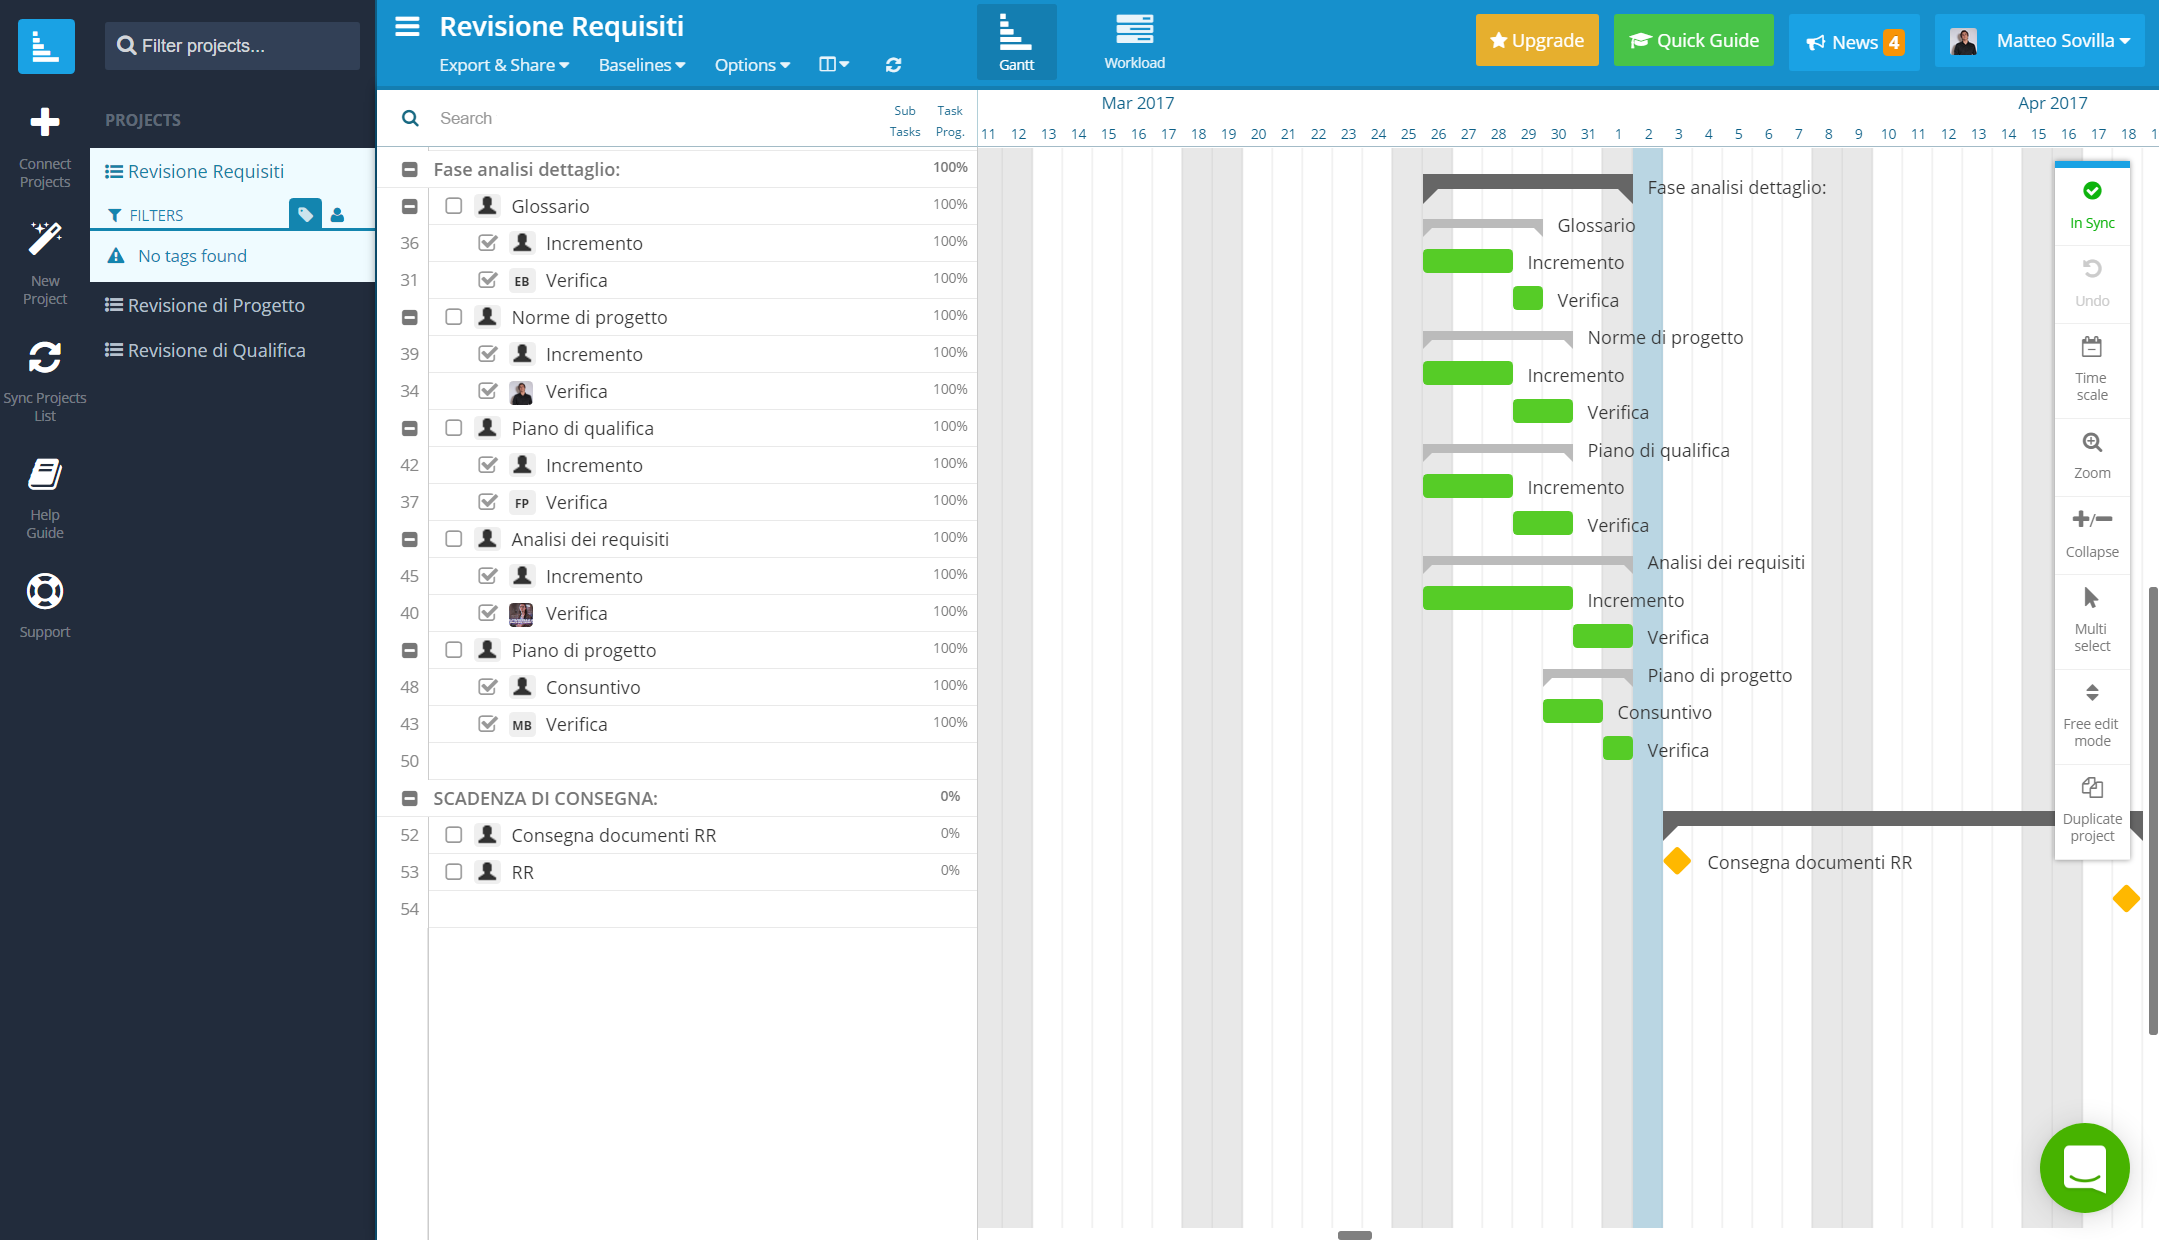
\includegraphics[scale=0.2]{./Immagini/Instagantt.png}
					\caption{Schermata principale dell'estensione Instagantt per Asana}\label{}
				\end{figure}
				\subsubsection{Norme di utilizzo}
				\paragraph{Creazione e assegnazione dei task\\}
					La gestione delle attività sarà effettuata utilizzando i task di Asana.
					All'inizio di ogni periodo del progetto, il \responsabilediprogetto\ si occuperà di creare i task corrispondenti alle attività individuate in fase di progettazione. Ciascun task riporterà una breve descrizione dell'attività rappresentata e l'indicazione sul periodo temporale ad essa assegnata. Durante l'avanzamento della progettazione si divideranno ricorsivamente i task in sotto-attività più semplici, fino a quando ciascun task potrà essere assegnato ad un'unica persona, prevedendone lo svolgimento in un periodo massimo di due giornate.
				\paragraph{Avanzamento delle attività\\}
					Al termine di ciascuna attività, il componente del gruppo ad essa assegnato è tenuto a cambiarne lo stato per indicarne il completamento. Per tutte le attività associabili a commit su GitHub, questo sarà fatto automaticamente all'atto del commit configurando Zapier come indicato al punto \ref{Zapier}. Nel caso di attività non tracciabili in questo modo sarà il componente preposto a dover aggiornare il task.
				\paragraph{Attività di verifica\\}
					Con la creazione dei task corrispondenti alle macro-attività di periodo, il \responsabilediprogetto\ assegnerà opportunamente ad essi uno o più \verificatori, in base al carico di lavoro atteso e alle disponibilità di ciascuno. \\
					I \verificatori\ sono gli unici componenti del gruppo, oltre al \responsabilediprogetto\ a cui è concesso creare dei task su Asana. Al termine della loro attività di verifica infatti sarà compito loro creare i task corrispondenti alle attività di correzione e associarvi i redattori corrispondenti. \\
					Il task corrispondente all'attività di verifica sarà segnato come completato dai \verificatori\ stessi nel momento in cui riterranno valido e conforme alle norme definite l'oggetto della loro verifica.
				\paragraph{Visualizzazione dei Task\\}
				Per vedere i task assegnati basta spostarsi nella pagina ``MY
				TASKS'' presente tra i link in alto a sinistra.\\
				Per avere una visione d'insieme sui task dell'intero gruppo basta
				spostarsi nella pagina ``Team Calendar'' presente nella tendina
				laterale. Da qui è possibile vedere le scadenze indicative disposte
				in un calendario.
				
		\subsection{Comunicazioni}
			\subsubsection{Esterne}
				Per le comunicazioni esterne è stata creata la casella di posta
				elettronica:
				\begin{center}
					\mailkaleidoscode
				\end{center}
				Tale indirizzo deve essere l'unico canale di comunicazione tra il
				gruppo di lavoro e l'esterno.
				Il \responsabilediprogetto\ è l'unico ad accedere
				all'indirizzo ed è quindi l'unico a poter comunicare con il Proponente ed il
				Committente del progetto. È compito del \responsabilediprogetto\ informare
				i membri del gruppo delle discussioni avvenute e,
				qualora fosse necessario, inoltrare loro il messaggio attraverso
				una \gl{mailing list}.
			\subsubsection{Interne}
				Per le comunicazioni interne viene utilizzato il sistema di
				comunicazione Slack.\\
				Tale sistema deve essere utilizzato dai membri del gruppo
				per comunicare tra loro.
				In questo modo, ogni componente è costantemente informato sullo
				scambio di informazioni interne.
				Qualora fosse necessario l'uso di e-mail, come ad esempio nel caso di
				un inoltro di messaggio da parte del \responsabilediprogetto,
				è stata creata una mailing list:
				\begin{center}
					\mailinglist
				\end{center}
				Per facilitare le comunicazioni tra i membri del gruppo, viene
				utilizzato anche il sistema di messaggistica e videoconferenza
				Google Hangout.
				L'uso di quest'ultimo, nel caso in cui
				vengano prese decisioni	o emergano contenuti utili allo
				sviluppo del progetto, comporta l'obbligo di redigere un verbale
				da parte di un membro del gruppo, che renderà disponibile attraverso
				Google Drive una volta terminata la conversazione.
				La verbalizzazione ha l'obiettivo di tenere
				traccia di ogni argomento discusso, in
				quanto una comunicazione verbale non documentata non è
				accettabile per il corretto svolgimento del progetto. Nel caso un verbale
				debba essere fornito in fase di revisione, sarà necessario stenderlo in \LaTeX\
				utilizzando il template fornito allo scopo.\\
				Anche per eventuali decisioni prese su Slack, si richiede che la conversazione
				venga documentata come sopra descritto.
			\subsection{Composizione e-mail}
				In questo paragrafo viene descritta la struttura che deve avere
				un messaggio sia per una comunicazione esterna che per una
				conversazione interna attraverso mailing list.
				\subsubsection{Destinatario}
					\begin{itemize}
						\item \textbf{Interno}: l'unico indirizzo utilizzabile è
						\mailkaleidoscode;
						\item \textbf{Esterno}: varia a seconda che ci si debba
						rivolgere  al Proponente, al \vardanega\ o al \cardin.
					\end{itemize}
				\subsubsection{Mittente}
					\begin{itemize}
						\item \textbf{Interno}: l'indirizzo di chi scrive
						il messaggio;
						\item \textbf{Esterno}: l'unico indirizzo utilizzabile è
						\mailkaleidoscode\ e deve essere usato solamente dal
						\responsabilediprogetto.
					\end{itemize}
				\subsubsection{Oggetto}
					L'oggetto deve essere chiaro ed esaustivo, possibilmente non
					confondibile con altri preesistenti.\\
					L'oggetto di una comunicazione, una volta avviata, non deve mai essere cambiato.\\
					Nel caso si debba comporre un messaggio di risposta vi è l'obbligo di aggiungere la
					particella ``Re:'' all'inizio dell'oggetto per poter distinguere i
					livelli di risposta; se si dovesse trattare di un inoltro, si deve
					usare invece la particella ``I:''.
				\subsubsection{Corpo}
					Il corpo di un messaggio deve contenere tutte le informazioni
					necessarie alla piena comprensione della comunicazione.\\
					Se alcune parti del messaggio hanno uno o più destinatari specifici,
					sarà necessario aggiungere il loro nome	prima del relativo paragrafo
					attraverso la segnatura	\textit{@destinatario}.\\
					In caso di risposta o inoltro del messaggio, il contenuto aggiunto deve
					essere sempre collocato in testa.
					Si consiglia di non cancellare il resto del messaggio,
					per consentire una visione completa della discussione.
				\subsubsection{Allegati}
					Qualora fosse necessario, è permesso l'invio di allegati.
			\subsection{Composizione di conversazioni su Slack}
				In questo paragrafo viene descritto come usare Slack per le conversazioni interne.\\
				È stato creato un canale Slack per ogni documento da redigere dove è possibile
				effettuare comunicazione di tematiche relative al documento oggetto del canale.\\
				È possibile creare un canale Slack per comunicare solamente con alcuni membri del
				gruppo qualora ce ne fosse bisogno.\\
				Se fosse necessario inviare un messaggio di struttura complessa (ad esempio, diviso
				per punti) è possibile inviare un post attraverso la funzionalità presente nella chat.\\
				Qualora si debbano inviare file o altri contenuti, è possibile allegarli al messaggio
				attraverso l'apposita funzionalità.\\
				Se fosse necessario riferirsi ad uno o più membri specifici di un canale, basterà
				aggiungere il loro nome prima della relativa comunicazione attraverso la segnatura
				\textit{@slackUsername}.
			\subsection{Riunioni}
				\subsubsection{Frequenza}
					Le riunioni interne del gruppo di lavoro avranno una cadenza settimanale.
				\subsubsection{Convocazione riunione}
					\paragraph{Interna\\}
						Il \responsabilediprogetto\ ha il compito di convocare le riunioni generali
						interne, ossia le riunioni a cui sono tenuti a partecipare tutti i membri
						del gruppo. Se un componente qualsiasi ritiene necessaria la convocazione di una
						riunione, deve inoltrare la richiesta al responsabile il quale decide se respingerla
						o accettarla. Il \responsabilediprogetto\ deve convocare l'assemblea con almeno
						quattro giorni di preavviso attraverso l'invio di un post su Slack nel canale
						dedicato, il cui corpo è formato da:
						\begin{itemize}
							\item Oggetto: Convocazione riunione n. X (dove X indica il numero progressivo
							di riunioni effettuate);
							\item Corpo:
							\begin{itemize}
								\item Data e ora prevista;
								\item Luogo previsto;
								\item Ordine del giorno.
							\end{itemize}
						\end{itemize}
						Ogni componente deve rispondere al messaggio nel minor tempo possibile confermando
						la presenza o in caso contrario motivando l'eventuale assenza.
						In caso di mancata risposta il \responsabilediprogetto\ è obbligato a contattare
						direttamente il componente che non ha fornito una risposta.
						Una volta ricevute tutte le risposte, il \responsabilediprogetto\
						può decidere se confermare, rinviare o annullare la riunione, basandosi sul numero di
						presenze e/o assenze, per garantire il maggior numero possibile di presenti.
						La conferma, il rinvio, l'annullamento devono essere notificati tramite messaggio
						nel canale di cui sopra.
					\paragraph{Esterna\\}
						Il \responsabilediprogetto\ ha il compito di convocare le riunioni generali esterne,
						ossia le riunioni a cui sono convocati tutti i membri del gruppo e
						il Proponente e/o Committente.
						Se un componente qualsiasi ritiene necessaria la convocazione di una riunione, deve
						inoltrare la richiesta al \responsabilediprogetto\ il quale decide se respingere o
						accettare tale richiesta.\\
						Il \responsabilediprogetto\ deve prima di tutto concordare con il Proponente e/o
						Committente le date e i luoghi possibili in cui svolgere la riunione attraverso
						l'invio di un'email contenente:
						\begin{itemize}
							\item Oggetto: Richiesta riunione;
							\item Corpo:
							\begin{itemize}
								\item Motivazione;
								\item Eventuali date e/o luoghi possibili.
							\end{itemize}
						\end{itemize}
						Dopodiché, il responsabile deve inviare un post ai
						membri del gruppo nel canale dedicato su Slack in cui sono specificate:
						\begin{itemize}
							\item Oggetto: Richiesta riunione col Proponente/Committente
							\item Corpo:
							\begin{itemize}
								\item Date e/o luoghi possibili.
							\end{itemize}
						\end{itemize}
						Ogni membro del gruppo deve rispondere alla comunicazione confermando la presenza o
						in caso contrario motivando l'eventuale essenza. In caso di mancata risposta, il
						\responsabilediprogetto\ deve contattare direttamente il componente che non ha
						fornito una risposta. Una volta ricevute tutte le risposte, il responsabile può
						decidere se confermare, rinviare, annullare la riunione con il Proponente/Committente
						basandosi sul numero di presenze e/o assenze.
						Il \responsabilediprogetto\ deve poi, in caso di:
						\begin{itemize}
							\item Conferma: comunicare a tutti i membri e al Proponente e/o Committente
							la data e il luogo definitivi;
							\item Rinvio: comunicare a tutti i membri la decisione presa e ripetere
							il procedimento dall'inizio;
							\item Annullamento: comunicare a tutti i membri la decisione presa e
							ripetere il procedimento dall'inizio.
						\end{itemize}
				\subsubsection{Svolgimento riunione}
					\paragraph{Esterna\\}
						All'inizio di ogni riunione, verificata la presenza dei membri previsti, viene scelto
						un segretario che avrà il compito di annotare gli argomenti trattati e di redigere
						il verbale della riunione, che dovrà poi essere caricato su Google Drive. 
						Tutti i partecipanti devono tenere un comportamento consono al miglior svolgimento
						dell'assemblea e al raggiungimento degli obbiettivi della stessa.
						Il segretario deve inoltre assicurarsi che venga seguito l'ordine del giorno
						in modo da affrontare ogni argomento previsto.
\end{document}